%%%%%%%%%%%%%%%%%%%%% {{{
%%Options for presentations (in-class) and handouts (e.g. print).
\documentclass[pdf,9pt]{beamer}
% \documentclass[pdf,9pt]{beamer}


%%%%%%%%%%%%%%%%%%%%%%
%Change this for different slides so it appears in bar
\usepackage{authoraftertitle}
\date{Chapter 3. Determinants and Diagonalization \\ \S 3-3. Diagonalization and Eigenvalues}

%%%%%%%%%%%%%%%%%%%%%%
%% Upload common style file
\usepackage{LyryxLAWASlidesStyle}

\begin{document}

%%%%%%%%%%%%%%%%%%%%%%%
%% Title Page and Copyright Common to All Slides

%Title Page
\input frontmatter/titlepage.tex

%LOTS Page
\input frontmatter/lyryxopentexts.tex

%Copyright Page
\input frontmatter/copyright.tex

%%%%%%%%%%%%%%%%%%%%%%%%% }}}
%--------------  -------------------------------%{{{ 2
\begin{frame}[fragile]
   \tableofcontents
\end{frame}
%-------------- end slide -------------------------------%}}}
\section[\textcolor{yellow}{}]{\textcolor{yellow}{Why Diagonalization?}}
%--------------  -------------------------------%{{{ 3
\frame{
\frametitle{Why Diagonalization?}
\pause
\begin{example}
    Let $A=
    \left[\begin{array}{rr}
        4  & -2 \\
        -1 & 3
    \end{array}\right]$.
    Find $A^{100}$.

    \uncover<2->{
    \begin{center}
    \alert{\Large How can we do this efficiently?}
    \end{center}}

    \uncover<3->{
    Consider the matrix
    $P=
    \left[\begin{array}{rr}
        1 & -2 \\
        1 & 1
    \end{array}\right]$.
    Observe that $P$ is invertible (why?), and that
    \[ P^{-1} =
    \frac{1}{3} \left[\begin{array}{rr}
        1 & 2 \\
        -1 & 1
    \end{array}\right].\]}

    \uncover<4->{
    Furthermore,
    \[ P^{-1}AP
    = \frac{1}{3} \left[\begin{array}{rr}
        1 & 2 \\
        -1 & 1
    \end{array}\right]
    \left[\begin{array}{rr}
        4 & -2 \\
        -1 & 3
    \end{array}\right]
    \left[\begin{array}{rr}
        1 & -2 \\
        1 & 1
    \end{array}\right]
    =
    \left[\begin{array}{rr}
        2 & 0 \\
        0 & 5
    \end{array}\right] = D,
    \]
    where $D$ is a \alert{diagonal} matrix.
    }
\end{example}
}
%-------------- end slide -------------------------------%}}}
%--------------  -------------------------------%{{{ 4
\frame{
\begin{example}[continued]
This is significant, because
\begin{eqnarray*}
P^{-1} A P & = & D \\
P(P^{-1} A P)P^{-1} & = & PDP^{-1} \\
(PP^{-1}) A (PP^{-1}) & = & PDP^{-1} \\
IAI & = & PDP^{-1} \\
A & = & PDP^{-1},
\end{eqnarray*}
\bigskip
\uncover<2->{
and so
\begin{eqnarray*}
A^{100} & = & (PDP^{-1})^{100} \\
& = & (PDP^{-1})(PDP^{-1})(PDP^{-1}) \cdots (PDP^{-1}) \\
& = & PD(P^{-1}P)D(P^{-1}P)D(P^{-1} \cdots P)DP^{-1} \\
& = & PDIDIDI \cdots I DP^{-1} \\
& = & PD^{100}P^{-1}.
\end{eqnarray*}
}
\end{example}
}
%-------------- end slide -------------------------------%}}}
%--------------  -------------------------------%{{{ 5
\frame{
\begin{example}[continued]
Now,
\[ D^{100} =
\left[\begin{array}{rr}
2 & 0 \\
0 & 5
\end{array}\right]^{100}
=
\left[\begin{array}{cc}
2^{100} & 0 \\
0 & 5^{100}
\end{array}\right].\]

Therefore,
\begin{eqnarray*}
A^{100} & = & PD^{100}P^{-1} \\
& = & \left[\begin{array}{rr}
1 & -2 \\
1 & 1
\end{array}\right]
\left[\begin{array}{cc}
2^{100} & 0 \\
0 & 5^{100}
\end{array}\right]
\left(\frac{1}{3}\right)
\left[\begin{array}{rr}
1 & 2 \\
-1 & 1
\end{array}\right] \\ \\
& = &
\frac{1}{3}
\left[\begin{array}{cc}
2^{100} + 2\cdot 5^{100} & 2^{100} - 2\cdot 5^{100} \\
2^{100} - 5^{100} & 2\cdot 2^{100} + 5^{100}
\end{array}\right] \\ \\
& = &
\frac{1}{3}
\left[\begin{array}{cc}
2^{100} + 2\cdot 5^{100} & 2^{100} - 2\cdot 5^{100} \\
2^{100} - 5^{100} & 2^{101} + 5^{100}
\end{array}\right].
\end{eqnarray*}
\myQED
\end{example}
}
%-------------- end slide -------------------------------%}}}
%--------------  -------------------------------%{{{ 6
\frame{
\begin{theorem}[Diagonalization and Matrix Powers]
If $A=PDP^{-1}$, then $A^k=PD^kP^{-1}$ for each
$k=1,2,3,\ldots$
\end{theorem}
\bigskip

\uncover<2->{
    \begin{emptytitle}
        The process of finding an \alert{invertible} matrix $P$ and
a \alert{diagonal} matrix $D$ so that $A=PDP^{-1}$
is referred to as \alert{diagonalizing} the matrix $A$,
and $P$ is called the \alert{diagonalizing} matrix for $A$.
    \end{emptytitle}
}
\bigskip

\uncover<3->{
\begin{problem}
\begin{itemize}
\item
When is it possible to diagonalize a matrix?
\item
How do we find a diagonalizing matrix?
\end{itemize}
\end{problem}}
}
%-------------- end slide -------------------------------%}}}
\section[\textcolor{yellow}{}]{\textcolor{yellow}{Eigenvalues and Eigenvectors}}
%--------------  -------------------------------%{{{ 7
\frame{
\frametitle{Eigenvalues and Eigenvectors}
\pause
\begin{definition}
    Let $A$ be an $n\times n$ matrix, $\lambda$ a real number,
    and $\vec{x}\neq \vec{0}$ an $n$-vector.
    If $A\vec{x}=\lambda \vec{x}$, then $\lambda$ is an
    \alert{eigenvalue} of $A$, and $\vec{x}$ is
    an \alert{eigenvector} of $A$ corresponding to $\lambda$,
    or a \alert{$\lambda$-eigenvector}.
\end{definition}
\pause
\vfill
\begin{example}
    Let $A=
    \left[\begin{array}{rr}
	1 & 2 \\
	1 & 2
    \end{array}\right]$ and
    $\vec{x}=\left[\begin{array}{r}
    1 \\ 1 \end{array}\right]$.
    Then
    \[ A\vec{x}=\left[\begin{array}{rr}
	1 & 2 \\
	1 & 2
    \end{array}\right]
    \left[\begin{array}{r} 1 \\ 1 \end{array}\right] =
    \left[\begin{array}{r} 3 \\ 3 \end{array}\right] =
    3 \left[\begin{array}{r} 1 \\ 1 \end{array}\right] =
    3\vec{x}.
    \]
    This means that $3$ is an \alert{eigenvalue} of $A$, and
    $\left[\begin{array}{r} 1 \\ 1 \end{array}\right]$ is an \alert{eigenvector of
    $A$ corresponding to $3$} (or a $3$-eigenvector of $A$).
\end{example}
}
%-------------- end slide -------------------------------%}}}
%--------------  -------------------------------%{{{ 8
\frame{
\begin{emptytitle}
    Suppose that $A$ is an $n\times n$ matrix, $\vec{x}\neq 0$ an $n$-vector,
    $\lambda\in\RR$, and that $A\vec{x}=\lambda \vec{x}$.
    \bigskip
    \pause

    Then
    \begin{eqnarray*}
	\lambda \vec{x} - A\vec{x}   & = & \vec{0} \\
	\lambda I \vec{x} - A\vec{x} & = & \vec{0} \\
	(\lambda I - A)\vec{x}       & = & \vec{0}
    \end{eqnarray*}
    \bigskip
    \pause

    Since $\vec{x}\neq \vec{0}$, the matrix $\lambda I-A$ has no inverse, and
    thus
    \[ \det(\lambda I-A)=0.\]
\end{emptytitle}
}
%-------------- end slide -------------------------------%}}}
%--------------  -------------------------------%{{{ 9
\frame{
\begin{definition}
    The \alert{characteristic polynomial} of an $n\times n$ matrix $A$ is
    \[ c_A(x)=\det(xI-A).\]
\end{definition}
\vfill
\pause
\begin{example}
    The characteristic polynomial of
    $A=\left[\begin{array}{rr}
    4 & -2 \\ -1 & 3
    \end{array}\right]$ is
    \begin{eqnarray*}
    c_A(x) & = & \det\left(
    \left[\begin{array}{rr}
    x & 0 \\ 0 & x
    \end{array}\right] -
    \left[\begin{array}{rr}
    4 & -2 \\ -1 & 3
    \end{array}\right]\right) \\
    & = & \det
    \left[\begin{array}{cc}
    x-4 & 2 \\ 1 & x-3
    \end{array}\right] \\
    & = & (x-4)(x-3)-2 \\
    & = & x^2-7x+10
    \end{eqnarray*}
\end{example}
}
%-------------- end slide -------------------------------%}}}
%--------------  -------------------------------%{{{ 10
\frame{
\begin{theorem}[Eigenvalues and Eigenvectors of a Matrix]
    Let $A$ be an $n\times n$ matrix.
    \begin{enumerate}
	\item The eigenvalues of $A$ are the \textcolor{yellow}{roots} of $c_A(x)$.
	\item The $\lambda$-eigenvectors $\vec{x}$ are the \textcolor{yellow}{nontrivial solutions} to $(\lambda I-A)\vec{x}= \vec{0}$.
    \end{enumerate}
\end{theorem}
\vfill
\pause
\begin{example}[continued]
    For $A=\left[\begin{array}{rr}
    4 & -2 \\ -1 & 3
    \end{array}\right]$, we have
    \[ c_A(x) =  x^2-7x+10 = (x-2)(x-5),\]
    so $A$ has eigenvalues $\lambda_1=2$ and $\lambda_2=5$.
    \bigskip
    \pause

    To find the $2$-eigenvectors of $A$, solve $(2I-A)\vec{x}= \vec{0}$:
    \[
    \left[\begin{array}{rr|r}
	-2 & 2  & 0 \\
	1  & -1 & 0
    \end{array}\right]
    \rightarrow
    \left[\begin{array}{rr|r}
	1  & -1 & 0 \\
	-2 & 2  & 0
    \end{array}\right]
    \rightarrow
    \left[\begin{array}{rr|r}
	1 & -1 & 0 \\
	0 & 0  & 0
    \end{array}\right]
    \]
\end{example}
}
%-------------- end slide -------------------------------%}}}
%--------------  -------------------------------%{{{ 11
\frame{
\begin{example}[continued]
The general solution, in parametric form, is
\[ \vec{x}=\left[\begin{array}{c}
t \\ t \end{array}\right] =
t\left[\begin{array}{c}
1 \\ 1 \end{array}\right]
\mbox{ where } t\in\RR. \]

\uncover<2->{To find the $5$-eigenvectors of $A$, solve $(5I-A)\vec{x}= \vec{0}$:
\[
\left[\begin{array}{rr|r}
1 & 2 & 0 \\
1 & 2 & 0
\end{array}\right]
\rightarrow
\left[\begin{array}{rr|r}
1 & 2 & 0 \\
0 & 0 & 0
\end{array}\right] \]}

\uncover<3->{
The general solution, in parametric form, is
\[ \vec{x}=\left[\begin{array}{r}
-2s \\ s \end{array}\right] =
s\left[\begin{array}{r}
-2 \\ 1 \end{array}\right]
\mbox{ where } s\in\RR. \]}
\end{example}
}
%-------------- end slide -------------------------------%}}}
%--------------  -------------------------------%{{{ 12
\frame{
\begin{definition}
    A \alert{basic eigenvector} of an $n\times n$ matrix $A$ is any
    nonzero multiple of a basic solution to $(\lambda I-A)\vec{x}= \vec{0}$, where
    $\lambda$ is an eigenvalue of $A$.
\end{definition}
\vfill
\pause
\begin{example}[continued]
    $\left[ \begin{array}{r} 1  \\ 1 \end{array}\right]$ and
    $\left[ \begin{array}{r} -2 \\ 1 \end{array}\right]$
    are basic eigenvectors of the matrix
    \[ A= \left[\begin{array}{rr}
	4  & -2 \\
	-1 & 3
    \end{array}\right] \]
    corresponding to eigenvalues $\lambda_1=2$ and $\lambda_2=5$, respectively.
\end{example}
}
%-------------- end slide -------------------------------%}}}
%--------------  -------------------------------%{{{ 13
\frame{
\begin{problem}
    For $A=
    \left[\begin{array}{rrr}
	3 & -4 & 2 \\
	1 & -2 & 2 \\
	1 & -5 & 5
    \end{array}\right]$,
    find $c_A(x)$, the eigenvalues of $A$, and the corresponding basic eigenvectors.
\end{problem}
\pause
\vfill
\begin{solution}
    \begin{align*}
	\det(xI-A) &=
	\left|\begin{array}{ccc}
	    x-3 & 4   & -2 \\
	    -1  & x+2 & -2 \\
	    -1  & 5   & x-5
	\end{array}\right|
	=
	\left|\begin{array}{ccc}
	    x-3 & 4   & -2   \\
	    0   & x-3 & -x+3 \\
	    -1  & 5   & x-5
    \end{array}\right| \\[0.5em]
	&=
	\left|\begin{array}{ccc}
	    x-3 & 4   & 2 \\
	    0   & x-3 & 0 \\
	    -1  & 5   & x
	\end{array}\right|
	= (x-3)
	\left|\begin{array}{ccc}
	    x-3 & 2 \\
	    -1  & x
    \end{array}\right|\\[0.5em]
	&= (x-3)(x^2-3x+2) = (x-3)(x-2)(x-1) = c_A(x).
    \end{align*}
\end{solution}
}
%-------------- end slide -------------------------------%}}}
%--------------  -------------------------------%{{{ 14
\frame{
\begin{solution}[continued]
    Therefore, the eigenvalues of $A$ are
    $\lambda_1=3, \lambda_2=2$, and $\lambda_3=1$.
    \bigskip
    \pause

    Basic eigenvectors corresponding to $\lambda_1=3$: solve
    $(3I-A)\vec{x}= \vec{0}$.
    \[ \left[\begin{array}{rrr|r}
	0  & 4 & -2 & 0 \\
	-1 & 5 & -2 & 0 \\
	-1 & 5 & -2 & 0
    \end{array}\right]
    \rightarrow \cdots \rightarrow
    \left[\begin{array}{rrr|r}
	1 & 0 & -\frac{1}{2} & 0 \\
	0 & 1 & -\frac{1}{2} & 0 \\
	0 & 0 & 0            & 0
    \end{array}
    \right]
    \]
    \pause

    Thus
    $\vec{x}=
    \left[\begin{array}{r}
	\frac{1}{2} t \\
	\frac{1}{2} t \\
	t
    \end{array}\right]
    =t
    \left[\begin{array}{r}
	\frac{1}{2} \\
	\frac{1}{2} \\
	1
    \end{array}\right]$, $t\in\RR$.
    \pause

    Choosing $t=2$ gives us
    $\vec{x}_1=
    \left[\begin{array}{r}
	1 \\ 1 \\ 2
    \end{array}\right]$
    as a basic eigenvector corresponding to $\lambda_1=3$.
\end{solution}
}
%-------------- end slide -------------------------------%}}}
%--------------  -------------------------------%{{{ 15
\frame{
\begin{solution}[continued]
    Basic eigenvectors corresponding to $\lambda_2=2$: solve
    $(2I-A)\vec{x}= \vec{0}$.
    \[ \left[\begin{array}{rrr|r}
	-1 & 4 & -2 & 0 \\
	-1 & 4 & -2 & 0 \\
	-1 & 5 & -3 & 0
    \end{array}\right]
    \rightarrow \cdots \rightarrow
    \left[\begin{array}{rrr|r}
	1 & 0 & -2 & 0 \\
	0 & 1 & -1 & 0 \\
	0 & 0 & 0  & 0
    \end{array}\right]
    \]
    \pause

    Thus
    $\vec{x}=
    \left[\begin{array}{r}
	2s \\
	s \\
	s
    \end{array}\right]
    =s
    \left[\begin{array}{r}
	2\\ 1\\ 1
    \end{array}\right]$, $s\in\RR$.
    \pause
    \bigskip

    Choosing $s=1$ gives us
    $\vec{x}_2=
    \left[\begin{array}{r}\vspace*{.02in}
	2 \\ 1 \\ 1
    \end{array}\right]$
    as a basic eigenvector corresponding to $\lambda_2=2$.
\end{solution}
}
%-------------- end slide -------------------------------%}}}
%--------------  -------------------------------%{{{ 16
\frame{
\begin{solution}[continued]
    Basic eigenvectors corresponding to $\lambda_3=1$: solve
    $(I-A)\vec{x}= \vec{0}$.
    \[ \left[\begin{array}{rrr|r}
	-2 & 4 & -2 & 0 \\
	-1 & 3 & -2 & 0 \\
	-1 & 5 & -4 & 0
    \end{array}\right]
    \rightarrow \cdots \rightarrow
    \left[\begin{array}{rrr|r}
	1 & 0 & -1 & 0 \\
	0 & 1 & -1 & 0 \\
	0 & 0 & 0  & 0
    \end{array}\right]
    \]
    \pause

    Thus
    $\vec{x}=
    \left[\begin{array}{r}
	r \\
	r \\
	r
    \end{array}\right]
    =r
    \left[\begin{array}{r}
	1\\ 1\\ 1
    \end{array}\right]$, $r\in\RR$.
    \pause
    \bigskip

    Choosing $r=1$ gives us
    $\vec{x}_3=
    \left[\begin{array}{r}
	1 \\ 1 \\ 1
    \end{array}\right]$
    as a basic eigenvector corresponding to $\lambda_3=1$.
    \myQED
\end{solution}
}
%-------------- end slide -------------------------------%}}}
\section[\textcolor{yellow}{}]{\textcolor{yellow}{Geometric Interpretation of Eigenvalues and Eigenvectors}}
%--------------  -------------------------------%{{{ 17
\frame{
\frametitle{Geometric Interpretation of Eigenvalues and Eigenvectors}
\pause
\begin{emptytitle}
    Let $A$ be a $2\times 2$ matrix.
    Then $A$ can be interpreted as a linear transformation from
    $\RR^2$ to $\RR^2$.
\end{emptytitle}
\vfill
\pause
\begin{problem}
    How does the linear transformation affect the eigenvectors
    of the matrix?
\end{problem}
\vfill
\pause
\begin{definition}
    Let $\vec{v}=\left[\begin{array}{c} a \\ b \end{array}\right]$ be a nonzero vector in $\RR^2$.
    Then $L_{\vec{v}}$ is the set of all scalar multiples of $\vec{v}$, i.e.,
    \[ L_{\vec{v}} = \RR \vec{v} =\left\{ t\vec{v} ~|~ t\in \RR \right\}.\]
\end{definition}
}
%-------------- end slide -------------------------------%}}}
%--------------  -------------------------------%{{{ 18
\begin{frame}[fragile]
    \begin{example}[revisited]
	$A=\begin{pmatrix} 4&-2\cr -1&3 \end{pmatrix} $ has two eigenvalues:
	$\lambda_1=2$ and $\lambda_2=5$ with corresponding eigenvectors
	\begin{align*}
	    \vec{v}_1 =\begin{pmatrix} 1\cr 1 \end{pmatrix}
	    \quad\text{and}\quad
	    \vec{v}_2 =\begin{pmatrix} -1\cr 1/2 \end{pmatrix}
	\end{align*}
    \end{example}
\end{frame}
%-------------- end slide -------------------------------%}}}
%--------------  -------------------------------%{{{ 19
\begin{frame}[fragile]
\begin{center}
    \begin{center}
        \begin{tikzpicture}[scale=0.7, transform shape]
        \tikzset{>=latex}
	\draw [->] (-5.5,0) -- (6.5,0) node [right] {$x$};
	\draw [->] (0,-4.5) -- (0,6.5) node [above] {$y$};
	\foreach \x in {-5,...,-1} {
	    \draw (\x,0.1) -- (\x,-0.1) node [below] {$\x$};
	}
	\foreach \x in {1,...,6} {
	    \draw (\x,0.1) -- (\x,-0.1) node [below] {$\x$};
	}
	\foreach \y in {-4,...,-1} {
	    \draw (0.1,\y) -- (-0.1,\y) node [left] {$\y$};
	}
	\foreach \y in {1,...,6} {
	    \draw (0.1,\y) -- (-0.1,\y) node [left] {$\y$};
	}

	\foreach \x in {-5,...,6}{
	    \draw [dotted,gray] (\x,-4.5) -- (\x,6.5);
	}
	\foreach \y in {-4,...,6}{
	    \draw [dotted,gray] (-5.5,\y) -- (6.5,\y);
	}
	\node at (3,7) {$A=\begin{pmatrix} 4&-2\cr -1&3 \end{pmatrix} $};
	\coordinate (A) at (4,-1);
	\coordinate (O) at (0,0);
	\coordinate (B) at (-2,3);
	\pause
	\draw [blue,->,thick] (O) -- (1,0);
	\pause
	\draw [red,->,thick] (O) -- (A);
	\pause
	\draw [blue,->,thick] (O) -- (0,1);
	\pause
	\draw [red,->,thick] (O) -- (B);
	\pause
	\begin{scope}
	    \clip(-5.5,-4.5) rectangle (6.5,6.5);
	    \foreach \i in {-2,0,2,4} {
		\draw [shorten >= -10cm,shorten <= -10cm,dashed,gray] (\i,\i)  -- +($(A)-(O)$);
		\draw [shorten >= -10cm,shorten <= -10cm,dashed,gray] (\i,\i)  -- +($(B)-(O)$);
		}
	    % \draw [shorten >= -10cm,shorten <= -10cm,dashed] (0,5)  -- +($(A)-(O)$);
	    % \draw [shorten >= -10cm,shorten <= -10cm,dashed] (0,5)  -- +($(B)-(O)$);
	\end{scope}
	\pause
	\draw [yellow,->] (0,0) -- (2,1);
	\pause
	\draw [magenta,->] (0,0) -- (6,1);
	\pause
	\draw [yellow,->] (0,0) -- (1,-1);
	\pause
	\draw [magenta,->] (0,0) -- (6,-4);
	\pause
	\draw [yellow,->] (0,0) -- (1,1);
	\pause
	\draw [magenta,->] (0,0) -- (2,2);
	\pause
	\draw [yellow,->] (0,0) -- (-1,0.5);
	\pause
	\draw [magenta,->] (0,0) -- (-5,2.5);
        % \coordinate (L) at (3.1,0.4);
        % \coordinate (P0) at (0.2,1.6);
        % \coordinate (0) at (0,0);
        % \coordinate (P) at (3,2.22);
        % \draw ($(P)!-1cm!(P0)$)  -- (P) node [below]  {$P$} -- (P0) node [above] {$P_0$} -- ($(P0)!-1cm!(P)$) node [left] {$L$};
        % \draw [thick,->,color=blue] (P0) --coordinate [pos={1/2}] (m) node [above] {${\vec{d}}$} ($(P)!1cm!(P0)$);
        % \draw[dashed,->] (0) node [below] {$} -- (P0);
        % \draw[dashed,->] (0) -- (P);
        % \filldraw (P) circle (0.05);
        % \filldraw (P0) circle (0.05);
        % \filldraw (0) circle (0.05);
        \end{tikzpicture}
    \end{center}
\end{center}
\end{frame}
%-------------- end slide -------------------------------%}}}
%--------------  -------------------------------%{{{ 20
\frame{
\begin{definition}
Let $A$ be a $2\times 2$ matrix and $L$ a line in $\RR^2$
through the origin.
Then $L$ is said to be \alert{$A$-invariant} if the vector
$A\vec{x}$ lies in $L$ whenever $\vec{x}$ lies in $L$,

\uncover<2->{
i.e., $A\vec{x}$ is a scalar multiple of $\vec{x}$,}

\uncover<3->{
i.e., $A\vec{x}=\lambda \vec{x}$ for some scalar $\lambda\in\RR$,}

\uncover<4->{
i.e., $\vec{x}$ is an eigenvector of $A$.}
\end{definition}
\bigskip

\uncover<5->{
\begin{theorem}[A-Invariance]
Let $A$ be a $2\times 2$ matrix and let $\vec{v}\neq 0$ be a vector in
$\RR^2$.
Then $L_{\vec{v}}$ is $A$-invariant if and only if $\vec{v}$ is an eigenvector
of $A$.
\end{theorem}}

}
%-------------- end slide -------------------------------%}}}
%--------------  -------------------------------%{{{ 21
\begin{frame}[fragile]
\begin{center}
    \begin{center}
        \begin{tikzpicture}[scale=0.7, transform shape]
        \tikzset{>=latex}
	\draw [->] (-5.5,0) -- (6.5,0) node [right] {$x$};
	\draw [->] (0,-4.5) -- (0,6.5) node [above] {$y$};
	\foreach \x in {-5,...,-1} {
	    \draw (\x,0.1) -- (\x,-0.1) node [below] {$\x$};
	}
	\foreach \x in {1,...,6} {
	    \draw (\x,0.1) -- (\x,-0.1) node [below] {$\x$};
	}
	\foreach \y in {-4,...,-1} {
	    \draw (0.1,\y) -- (-0.1,\y) node [left] {$\y$};
	}
	\foreach \y in {1,...,6} {
	    \draw (0.1,\y) -- (-0.1,\y) node [left] {$\y$};
	}

	\foreach \x in {-5,...,6}{
	    \draw [dotted,gray] (\x,-4.5) -- (\x,6.5);
	}
	\foreach \y in {-4,...,6}{
	    \draw [dotted,gray] (-5.5,\y) -- (6.5,\y);
	}
	\node at (3,7) {$A=\begin{pmatrix} 4&-2\cr -1&3 \end{pmatrix} $};
	\coordinate (A) at (4,-1);
	\coordinate (O) at (0,0);
	\coordinate (B) at (-2,3);
	% \pause
	\draw [blue,->,thick] (O) -- (1,0);
	% \pause
	\draw [red,->,thick] (O) -- (A);
	% \pause
	\draw [blue,->,thick] (O) -- (0,1);
	% \pause
	\draw [red,->,thick] (O) -- (B);
	% \pause
	\begin{scope}
	    \clip(-5.5,-4.5) rectangle (6.5,6.5);
	    \foreach \i in {-2,0,2,4} {
		\draw [shorten >= -10cm,shorten <= -10cm,dashed,gray] (\i,\i)  -- +($(A)-(O)$);
		\draw [shorten >= -10cm,shorten <= -10cm,dashed,gray] (\i,\i)  -- +($(B)-(O)$);
		}
	\end{scope}
	% \pause
	% \draw [yellow,->] (0,0) -- (2,1);
	% \pause
	% \draw [magenta,->] (0,0) -- (6,1);
	% \pause
	% \draw [yellow,->] (0,0) -- (1,-1);
	% \pause
	% \draw [magenta,->] (0,0) -- (6,-4);
	% \pause
	\draw [yellow,->] (0,0) -- (1,1);
	% \pause
	\draw [magenta,->] (0,0) -- (2,2);
	% \pause
	\draw [yellow,->] (0,0) -- (-1,0.5);
	% \pause
	\draw [magenta,->] (0,0) -- (-5,2.5);
	\pause
	\begin{scope}
	    \clip(-5.5,-4.5) rectangle (6.5,6.5);
	    \draw [shorten >= -10cm,shorten <= -10cm,purple,very thick] (0,0) -- (1,1);
	    \pause
	    \draw [shorten >= -10cm,shorten <= -10cm,purple,very thick] (0,0) --(-2,1);
	\end{scope}
        \end{tikzpicture}
    \end{center}
\end{center}
\end{frame}
%-------------- end slide -------------------------------%}}}
%--------------  -------------------------------%{{{ 22
\frame{
\begin{problem}
Let $m\in\RR$ and consider the linear transformation
$Q_m : \RR^2 \rightarrow \RR^2$,
i.e., reflection in the line $y=mx$.
\begin{center}
    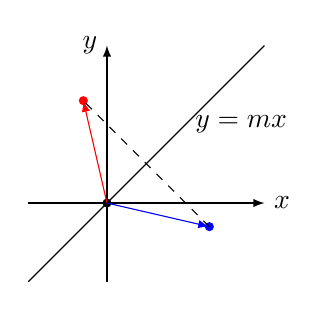
\begin{tikzpicture}[scale=1, transform shape]
	\tikzset{>=latex}
	\coordinate (P) at (1.3,-0.3);
	\coordinate (Q) at (-0.3,1.3);
	\coordinate (0) at (0,0);
	\draw [->] (-1,0) -- (2,0) node [right] {$x$};
	\draw [->] (0,-1) -- (0,2) node [left] {$y$};
	\filldraw (0) circle (0.05);
	\filldraw [blue] (P) circle (0.05);
	\draw [->,blue] (0) -- (P);
	\draw [->,red] (0) -- (Q);
	\filldraw[red] (Q) circle (0.05);
	\draw (-1,-1) -- (1,1) node [right] {$y=mx$} -- (2,2);
	\draw [dashed] (P) -- (Q);
    \end{tikzpicture}
\end{center}
Recall that this is a matrix transformation induced by
\[
    A=\frac{1}{1+m^2}
    \left[\begin{array}{cc}
	    1-m^2 & 2m \\
	    2m & m^2-1
    \end{array}\right].
\]
Find the lines that pass through origin and are $A$-invariant.
Determine corresponding eigenvalues.
\end{problem}



}
%-------------- end slide -------------------------------%}}}
%--------------  -------------------------------%{{{ 23
\begin{frame}[fragile]
\begin{solution}
\begin{center}
    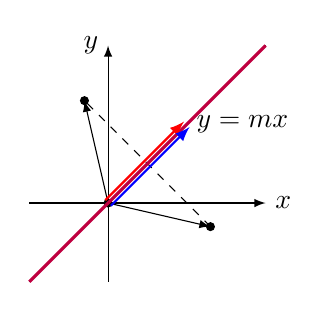
\begin{tikzpicture}[scale=1, transform shape]
	\tikzset{>=latex}
	\coordinate (P) at (1.3,-0.3);
	\coordinate (Q) at (-0.3,1.3);
	\coordinate (0) at (0,0);
	\draw [->] (-1,0) -- (2,0) node [right] {$x$};
	\draw [->] (0,-1) -- (0,2) node [left] {$y$};
	\filldraw (0) circle (0.05);
	\filldraw  (P) circle (0.05);
	\draw [->] (0) -- (P);
	\draw [->] (0) -- (Q);
	\filldraw (Q) circle (0.05);
	\draw (-1,-1) -- (1,1) node [right] {$y=mx$} -- (2,2);
	\draw [dashed] (P) -- (Q);
	\pause
	\draw [very thick,purple] (-1,-1) -- (2,2);
	\pause
	\draw [->,red,yshift=0.1em,xshift=-0.1em,thick] (0,0) -- (1,1);
	\pause
	\draw [->,blue,yshift=-0.1em,xshift=0.1em,thick] (0,0) -- (1,1);
	% \pause
	% \draw [very thick,purple] (-1,1) -- (1,-1);
    \end{tikzpicture}
\end{center}
\pause
\uncover<5->{
Let $\vec{x}_1=\left[\begin{array}{c}
1 \\ m \end{array}\right]$. Then $L_{\vec{x}_1}$ is $A$-invariant, that is, $\vec{x}_1$ is an eigenvector.
Since the vector won't change, its eigenvalue should be $1$. Indeed, one can verify that
\begin{align*}
    A \vec{x}_1 =
    \frac{1}{1+m^2}
    \left[\begin{array}{cc}
	1-m^2 & 2m \\
	2m    & m^2-1
    \end{array}\right]
    \begin{pmatrix} 1\cr m \end{pmatrix}
    = ... =
    \begin{pmatrix} 1\cr m \end{pmatrix}
    =
    \vec{x}_1.
\end{align*}
}
\end{solution}
\end{frame}

\begin{frame}[fragile]
    \begin{solution}[continued]
\begin{center}
    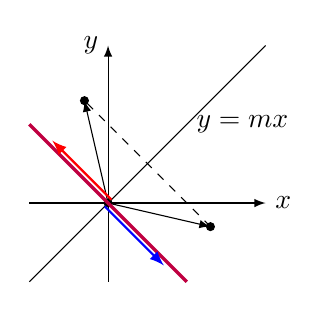
\begin{tikzpicture}[scale=1, transform shape]
	\tikzset{>=latex}
	\coordinate (P) at (1.3,-0.3);
	\coordinate (Q) at (-0.3,1.3);
	\coordinate (0) at (0,0);
	\draw [->] (-1,0) -- (2,0) node [right] {$x$};
	\draw [->] (0,-1) -- (0,2) node [left] {$y$};
	\filldraw (0) circle (0.05);
	\filldraw  (P) circle (0.05);
	\draw [->] (0) -- (P);
	\draw [->] (0) -- (Q);
	\filldraw (Q) circle (0.05);
	\draw (-1,-1) -- (1,1) node [right] {$y=mx$} -- (2,2);
	\draw [dashed] (P) -- (Q);
	\pause
	\draw [very thick,purple] (-1,1) -- (1,-1);
	% \draw [very thick,purple] (-1,-1) -- (2,2);
	\pause
	\draw [->,red,thick,xshift=0.12em,yshift=0.12em] (0,0) -- (-0.75,0.75);
	\pause
	\draw [->,blue,thick,xshift=-0.12em,yshift=-0.12em] (0,0) -- (0.75,-0.75);
    \end{tikzpicture}
\end{center}
\pause
\uncover<5->{
Let $\vec{x}_2=\left[\begin{array}{c}
-m \\ 1 \end{array}\right]$. Then $L_{\vec{x}_2}$ is $A$-invariant, that is, $\vec{x}_2$ is an eigenvector.
Since the vector won't change the size, only flip the direction, its eigenvalue should be $-1$. Indeed, one can verify that
\begin{align*}
    A \vec{x}_2 =
    \frac{1}{1+m^2}
    \left[\begin{array}{cc}
	1-m^2 & 2m \\
	2m    & m^2-1
    \end{array}\right]
    \begin{pmatrix} -m\cr 1 \end{pmatrix}
    = \cdots =
    \begin{pmatrix} m\cr -1 \end{pmatrix}
    =
    - \vec{x}_2.
\end{align*}
\myQED
}
\end{solution}
\end{frame}
%-------------- end slide -------------------------------%}}}
% %--------------  -------------------------------%{{{ 24
% \frame{
% \begin{example}[continued]
% More generally, any vector
% $\left[\begin{array}{c}
% k \\ km \end{array}\right]$, $k\neq 0$,
% lies in the line $y=mx$ and is an eigenvector of $A$.
%
% Another way of saying this is that the line $y=mx$ is $A$-invariant
% for the matrix
% \[ A=
%     \frac{1}{1+m^2}
% \left[\begin{array}{cc}
%     1-m^2 & 2m \\
%     2m    & m^2-1
% \end{array}\right].\]
% \end{example}
% }
% %-------------- end slide -------------------------------%}}}
%--------------  -------------------------------%{{{ 25
\frame{
\begin{example}
Let $\theta$ be a real number, and
$R_{\theta} : \RR^2 \rightarrow \RR^2$
rotation through an angle of $\theta$, induced by the matrix
\[ A=
\left[\begin{array}{cc}
\cos\theta & -\sin\theta \\
\sin\theta & \cos\theta
\end{array}\right].\]

\vspace{1em}
\pause
{\bf \textcolor{lgtblue}{Claim:}}
$A$ has no real eigenvalues unless $\theta$ is an integer multiple of $\pi$, i.e.,
$\pm\pi, \pm 2\pi, \pm 3\pi$, etc.
\bigskip

\vspace{3em}
\pause
Consequence: a line $L$ in $\RR^2$ is $A$ invariant
if and only if $\theta$ is an integer multiple of $\pi$.
\end{example}
}
%-------------- end slide -------------------------------%}}}
\section[\textcolor{yellow}{}]{\textcolor{yellow}{Diagonalization}}
%--------------  -------------------------------%{{{ 26
\frame{
\frametitle{Diagonalization}
\pause
\begin{emptytitle}
    Denote an $n\times n$ diagonal matrix by
    \begin{align*}
	\diag(a_1, a_2, \ldots, a_n)
	=
	\left[\begin{array}{cccccc}
	    a_1    & 0      & 0      & \cdots & 0       & 0 \\
	    0      & a_2    & 0      & \cdots & 0       & 0 \\
	    0      & 0      & a_3    & \cdots & 0       & 0 \\
	    \vdots & \vdots & \vdots & \vdots & \vdots  & \vdots \\
	    0      & 0      & 0      & \cdots & a_{n-1} & 0\\
	    0      & 0      & 0      & \cdots & 0       & a_n
	\end{array}\right]
    \end{align*}
    \bigskip
    \pause

    {\bf Recall} that if $A$ is an $n\times n$ matrix and $P$
    is an invertible $n\times n$ matrix so that $P^{-1}AP$ is
    diagonal, then $P$ is called a
    \alert{diagonalizing matrix} of $A$, and $A$ is
    \alert{diagonalizable}.
\end{emptytitle}
}
%-------------- end slide -------------------------------%}}}
%--------------  -------------------------------%{{{ 27
\begin{frame}[fragile]
\begin{emptytitle}
 \begin{itemize}
    \item Suppose we have $n$ eigenvalue-eigenvector pairs:
	\begin{align*}
	    A \vec{x}_j = \lambda_j \vec{x}_j\,, \quad j = 1, 2, \ldots, n
	\end{align*}
	\bigskip
	\pause
	\vfill
    \item Pack the above $n$ columns vectors into a matrix:\\[1em]
	\begin{eqnarray*}
	    \textcolor{red}{\left[ \begin{array}{c|c|c|c} A\vec{x}_1 & A\vec{x}_2 & \cdots & A\vec{x}_n \end{array} \right]} & \textcolor{red}{=} &
	    \textcolor{red}{\left[ \begin{array}{c|c|c|c}
	    \lambda_1\vec{x}_1 &
	    \lambda_2\vec{x}_2 &
	    \cdots &
	    \lambda_n\vec{x}_n \end{array} \right]} \\
	    ||\hspace{ 5em } 		 &&\\
	    \textcolor{red}{A} \: \textcolor{yellow}{\left[ \begin{array}{c|c|c|c} \vec{x}_1 &  \vec{x}_2  & \cdots &  \vec{x}_n \end{array} \right]}
	    &  & \hspace{4em}||
	\end{eqnarray*}
	\begin{align*}
	    \hspace{9em}
	    \textcolor{yellow}{\left[ \begin{array}{c|c|c|c} \vec{x}_1 &  \vec{x}_2  & \cdots &  \vec{x}_n \end{array} \right]}
	    \textcolor{blue}{\left[ \begin{array}{cccc} \lambda_1 & & & \\ & \lambda_2 & & \\ & & \ddots & \\ & & & \lambda_n \end{array} \right]}
	\end{align*}
\end{itemize}
\end{emptytitle}
\end{frame}
%-------------- end slide -------------------------------%}}}
%--------------  -------------------------------%{{{ 28
\begin{frame}[fragile]
\begin{emptytitle}
\begin{itemize}
    \item By denoting:
	\begin{align*}
	     \textcolor{yellow}{   P = \left[ \begin{array}{c|c|c|c} \vec{x}_1 &  \vec{x}_2  & \cdots &  \vec{x}_n \end{array} \right]}
	     \quad \mbox{and} \quad
	     \textcolor{blue}{D = \diag\left(\lambda_1,\cdots,\lambda_n\right)}
	    % \left[ \begin{array}{cccc} \lambda_1 & & & \\ & \lambda_2 & & \\ & & \ddots & \\ & & & \lambda_n \end{array} \right]
	\end{align*}
	we see that
	\begin{align*}
	    \textcolor{red}{A} \textcolor{yellow}{P} = \textcolor{yellow}{P} \textcolor{blue}{D}
	\end{align*}
	\vspace{4em}
	\pause

    \item Hence, provided $ \textcolor{yellow}{P}$ is invertible, we have \\[0.5em]
	\begin{align*}
	    \textcolor{red}{A}  = \textcolor{yellow}{P} \textcolor{blue}{D}\textcolor{yellow}{P}^{-1}
	    \quad\text{or equivalently}\quad
	    \textcolor{blue}{D}  = \textcolor{yellow}{P}^{-1} \textcolor{red}{A} \textcolor{yellow}{P}\\[0.5em]
	\end{align*}
	\pause
	that is, $\textcolor{red}{A}$ is diagonalizable.
\end{itemize}
\end{emptytitle}
\end{frame}
%-------------- end slide -------------------------------%}}}
%--------------  -------------------------------%{{{ 29
\frame{
\begin{theorem}[Matrix Diagonalization]
    Let $A$ be an $n\times n$ matrix.
    \begin{enumerate}
    \item $A$ is diagonalizable if and only if it has eigenvectors $\vec{x}_1, \vec{x}_2, \ldots, \vec{x}_n$ so that
	\begin{align*}
	    \textcolor{yellow}{P = \left[
	    \begin{array}{cccc}
		\vec{x}_1 & \vec{x}_2 & \cdots & \vec{x}_n
	    \end{array}\right]}
	\end{align*}
	is invertible.
    \item<2-> If $P$ is invertible, then
	\begin{align*}
	    \textcolor{yellow}{P}^{-1} \textcolor{red}{A} \textcolor{yellow}{P} = \textcolor{blue}{\diag(\lambda_1, \lambda_2, \ldots, \lambda_n ) }
	\end{align*}
	where $\lambda_i$ is the eigenvalue of $A$ corresponding to
	the eigenvector $\vec{x}_i$, i.e., $A\vec{x}_i=\lambda_i \vec{x}_i$.
    \end{enumerate}
\end{theorem}
}
%-------------- end slide -------------------------------%}}}
%--------------  -------------------------------%{{{ 30
\frame{
\begin{example}
$A=
\left[\begin{array}{rrr}
3 & -4 & 2 \\
1 & -2 & 2 \\
1 & -5 & 5
\end{array}\right]$ has eigenvalues and
corresponding basic eigenvectors
\begin{align*}
    \lambda_1=3\quad\text{and}\quad
    \vec{x}_1 = \left[\begin{array}{r}
	    1 \\ 1 \\ 2
    \end{array}\right];\\
    \lambda_2=2\quad\text{and}\quad
    \vec{x}_2 = \left[\begin{array}{r}
	    2 \\ 1 \\ 1
    \end{array}\right];\\
    \lambda_3=1\quad\text{and}\quad
    \vec{x}_3 = \left[\begin{array}{r}
	    1 \\ 1 \\ 1
    \end{array}\right].
\end{align*}

\end{example}
}
%-------------- end slide -------------------------------%}}}
%--------------  -------------------------------%{{{ 31
\begin{frame}[fragile]
    \begin{example}[continued]
	    Let
	    $P= \left[
	    \begin{array}{ccc}
	    \vec{x}_1 & \vec{x}_2 & \vec{x}_3
	    \end{array}\right]
	    =\left[\begin{array}{rrr}
	    1 & 2 & 1 \\
	    1 & 1 & 1 \\
	    2 & 1 & 1
	    \end{array}\right]$.
      \pause
      Then $P$ is invertible, so by the above Theorem,
      \[ P^{-1}AP=\diag(3,2,1) = \left[\begin{array}{rrr}
              3 & 0 & 0 \\
              0 & 2 & 0 \\
              0 & 0 & 1
      \end{array}\right].\]
      \myQED
    \end{example}
\end{frame}
%-------------- end slide -------------------------------%}}}
%--------------  -------------------------------%{{{ 32
\frame{
  \begin{remark}
    It is not always possible to find $n$ eigenvectors so that $P$ is invertible.
  \end{remark}

\medskip
\pause
\begin{example}
Let $A=
\left[\begin{array}{rrr}
        1 & -2 & 3 \\
        2 & 6 & -6 \\
        1 & 2 & -1
\end{array}\right]$.

\pause
Then
\[ c_A(x) =
    \left|\begin{array}{ccc}
        x-1 & 2 & -3 \\
        -2 & x-6 & 6 \\
        -1 & -2 & x+1
    \end{array}\right|
    = \cdots = (x-2)^3.
\]

\pause
$A$ has only one eigenvalue, $\lambda_1=2$, with multiplicity three. Sometimes,
one writes
\begin{align*}
    \lambda_1=\lambda_2=\lambda_3=2.
\end{align*}
\end{example}
}
%-------------- end slide -------------------------------%}}}
%--------------  -------------------------------%{{{ 33
\frame{
\begin{example}[continued]
To find the $2$-eigenvectors of $A$, solve the system $(2I-A)\vec{x}= \vec{0}$.
\[
\left[\begin{array}{rrr|r}
    1  & 2  & -3 & 0 \\
    -2 & -4 & 6  & 0 \\
    -1 & -2 & 3  & 0
\end{array}\right]
\rightarrow \cdots \rightarrow
\left[\begin{array}{rrr|r}
    1 & 2 & -3 & 0 \\
    0 & 0 & 0  & 0 \\
    0 & 0 & 0  & 0
\end{array}\right]
\]

\pause
The general solution in parametric form is
\[ \vec{x} =
    \left[\begin{array}{c}
            -2s+3t \\ s \\ t
    \end{array}\right]
    =s\left[\begin{array}{r}
            -2 \\ 1 \\ 0
    \end{array}\right]
    +
    t\left[\begin{array}{r}
            3 \\ 0 \\ 1
    \end{array}\right],\quad s,t\in\RR.
\]

\pause
Since the system has only {\bf two} basic solutions, there
are only two basic eigenvectors, implying that the matrix
$A$ is {\bf not diagonalizable}.
\myQED
\end{example}
}
%-------------- end slide -------------------------------%}}}
%--------------  -------------------------------%{{{ 34
\frame{
\begin{problem}
Diagonalize, if possible, the matrix
$A=\left[\begin{array}{rrr}
    1 & 0 & 1 \\
    0 & 1 & 0 \\
    0 & 0 & -3
\end{array}\right]$.
\end{problem}
\pause
\vfill
\begin{solution}
\[ c_A(x)=\det(xI-A) =
    \left|\begin{array}{ccc}
        x-1 & 0 & -1 \\
        0 & x-1 & 0 \\
        0 & 0 & x+3
    \end{array}\right|
    =(x-1)^2(x+3).
\]

\pause
$A$ has eigenvalues $\lambda_1=1$ of multiplicity two;
$\lambda_2=-3$ of multiplicity one.
\end{solution}
}
%-------------- end slide -------------------------------%}}}
%--------------  -------------------------------%{{{ 35
\frame{
\begin{solution}[continued]
Eigenvectors for $\lambda_1=1$: solve $(I-A)\vec{x}= \vec{0}$.
\[ \left[\begin{array}{rrr|r}
0 & 0 & -1 & 0 \\
0 & 0 & 0 & 0 \\
0 & 0 & 4 & 0
\end{array}\right]
\rightarrow
\left[\begin{array}{rrr|r}
0 & 0 & 1 & 0 \\
0 & 0 & 0 & 0 \\
0 & 0 & 0 & 0
\end{array}\right]
\]

\uncover<2->{
$\vec{x} = \left[\begin{array}{r} s \\ t \\ 0
\end{array}\right]$, $s,t\in\RR$
so basic eigenvectors corresponding to $\lambda_1=1$ are}

\uncover<3->{
\[
\left[\begin{array}{r} 1 \\ 0 \\ 0
\end{array}\right],
\left[\begin{array}{r} 0 \\ 1 \\ 0
\end{array}\right]
\]}
\end{solution}
}
%-------------- end slide -------------------------------%}}}
%--------------  -------------------------------%{{{ 36
\frame{
\begin{solution}[continued]
Eigenvectors for $\lambda_2=-3$: solve $(-3I-A)\vec{x}= \vec{0}$.
\[ \left[\begin{array}{rrr|r}
    -4 & 0  & -1 & 0 \\
    0  & -4 & 0  & 0 \\
    0  & 0  & 0  & 0
\end{array}\right]
\rightarrow
\left[\begin{array}{rrr|r}
    1 & 0 & \frac{1}{4} & 0 \\
    0 & 1 & 0           & 0 \\
    0 & 0 & 0           & 0
\end{array}\right]
\]
\uncover<2->{
$\vec{x} = \left[\begin{array}{c} -\frac{1}{4}t \\ 0 \\ t
\end{array}\right]$, $t\in\RR$
so a basic eigenvector corresponding to $\lambda_2=-3$ is
\[
\left[\begin{array}{r} -1 \\ 0 \\ 4
\end{array}\right]
\]}
\end{solution}
}
%-------------- end slide -------------------------------%}}}
%--------------  -------------------------------%{{{ 37
\frame{
\begin{solution}[continued]
Let
\[ P= \left[\begin{array}{ccc}
    -1 & 1 & 0 \\
    0  & 0 & 1 \\
    4  & 0 & 0
\end{array}\right].
\]

\pause
Then $P$ is invertible,
\pause and
\[ P^{-1}AP=\diag(-3,1,1)=
    \left[\begin{array}{ccc}
            -3 & 0 & 0 \\
            0  & 1 & 0 \\
            0  & 0 & 1
    \end{array}\right].
\]
\myQED
\end{solution}
}
%-------------- end slide -------------------------------%}}}
%--------------  -------------------------------%{{{ 38
\frame{
\begin{theorem}[Matrix Diagonalization Test]
A square matrix $A$ is diagonalizable if and only if every
eigenvalue $\lambda$ of multiplicity $m$ yields exactly $m$
basic eigenvectors, i.e., the solution to
$(\lambda I-A)\vec{x}= \vec{0}$ has $m$ parameters.
\end{theorem}
\bigskip

\uncover<2->{
    \begin{emptytitle}
A special case of this is:
    \end{emptytitle}
\begin{theorem}[Distinct Eigenvalues and Diagonalization]
An $n\times n$ matrix with distinct eigenvalues is diagonalizable.
\end{theorem}}
}
%-------------- end slide -------------------------------%}}}
%--------------  -------------------------------%{{{ 39
\frame{
\begin{problem}
Show that
$A=
\left[\begin{array}{ccc}
1 & 1 & 0 \\
0 & 1 & 0 \\
0 & 0 & 2
\end{array}\right]$
is not diagonalizable.
\end{problem}
\vfill

\pause
\begin{solution}
First,
\[ c_A(x) =
    \left|\begin{array}{ccc}
        x-1 & -1 & 0 \\
        0 & x-1 & 0 \\
        0 & 0 & x-2
    \end{array}\right|
    = (x-1)^2(x-2),
\]
so $A$ has eigenvalues $\lambda_1=1$ of multiplicity two;
$\lambda_2=2$ (of multiplicity one).
\end{solution}
}
%-------------- end slide -------------------------------%}}}
%--------------  -------------------------------%{{{ 40
\frame{
\begin{solution}[continued]
Eigenvectors for $\lambda_1=1$: solve $(I-A)\vec{x}= \vec{0}$.
\[ \left[\begin{array}{rrr|r}
    0 & -1 & 0 & 0 \\
    0 & 0 & 0 & 0 \\
    0 & 0 & -1 & 0
\end{array}\right]
\rightarrow
\left[\begin{array}{rrr|r}
    0 & 1 & 0 & 0 \\
    0 & 0 & 1 & 0 \\
    0 & 0 & 0 & 0
\end{array}\right]
\]

\pause
Therefore,
$\vec{x} = \left[\begin{array}{r} s \\ 0 \\ 0 \end{array}\right]$, $s\in\RR$.
\bigskip
\pause

Since $\lambda_1=1$ has multiplicity two, but has only one basic eigenvector, we can conclude that $A$ is NOT diagonalizable.
\myQED
\end{solution}
}
%-------------- end slide -------------------------------%}}}
\section[\textcolor{yellow}{}]{\textcolor{yellow}{Linear Dynamical Systems}}
%--------------  -------------------------------%{{{ 41
\frame{
\frametitle{Linear Dynamical Systems}
\pause
\begin{definition}
    A \alert{linear dynamical system} consists of
    \begin{itemize}
	\item[--] an $n\times n$ matrix $A$ and an $n$-vector $\vec{v}_0$; \pause
	\item[--] a \alert{matrix recursion} defining $\vec{v}_1, \vec{v}_2, \vec{v}_3, \ldots$ by $\vec{v}_{k+1}=A\vec{v}_k$; i.e.,
	    \pause
	    \begin{eqnarray*}
		\vec{v}_1 & =      & A\vec{v}_0                                \\
		\vec{v}_2 & =      & A\vec{v}_1 = A(A\vec{v}_0)=A^2\vec{v}_0   \\
		\vec{v}_3 & =      & A\vec{v}_2 = A(A^2\vec{v}_0)=A^3\vec{v}_0 \\
		\vdots    & \vdots & \vdots                                    \\
		\vec{v}_k & =      & A^k\vec{v}_0.
	    \end{eqnarray*}
    \end{itemize}
\end{definition}
\pause
\vfill
\begin{remark}
    Linear dynamical systems are used, for example, to model the evolution of populations over time.
\end{remark}
}
%-------------- end slide -------------------------------%}}}
%--------------  -------------------------------%{{{ 42
\frame{
\begin{emptytitle}
    If $A$ is diagonalizable, then
    \[ P^{-1}AP=D=\diag( \lambda_1, \lambda_2, \ldots, \lambda_n),\]
    where $\lambda_1, \lambda_2, \ldots, \lambda_n$ are the
    (not necessarily distinct) eigenvalues of $A$.
    \bigskip
    \pause

    Thus $A=PDP^{-1}$, and $A^k=PD^kP^{-1}$.  Therefore,
    \[\vec{v}_k = A^k\vec{v}_0 = PD^kP^{-1}\vec{v}_0.\]
\end{emptytitle}
}
%-------------- end slide -------------------------------%}}}
%--------------  -------------------------------%{{{ 43
\frame{
\begin{problem}
Consider the linear dynamical system $\vec{v}_{k+1}=A\vec{v}_k$ with
\[
A=\left[\begin{array}{rr}
    2 & 0 \\
    3 & -1
\end{array}\right], \quad\text{and}\quad
\vec{v}_0 =\left[\begin{array}{r}
1 \\ -1
\end{array}\right].\]
Find a formula for $\vec{v}_k$.
\end{problem}
\vfill
\pause
\begin{solution}
First,
$c_A(x)=(x-2)(x+1)$, so $A$ has eigenvalues $\lambda_1=2$ and $\lambda_2=-1$, and thus is diagonalizable.
\bigskip

\pause
Solve $(2I-A)\vec{x}= \vec{0}$:
\[ \left[\begin{array}{cc|c}
        0  & 0 & 0 \\
        -3 & 3 & 0
    \end{array}\right]
    \rightarrow
    \left[\begin{array}{cc|c}
        1 & -1 & 0 \\
        0 & 0  & 0
    \end{array}\right]\]
    has general solution
    $\vec{x}=\left[\begin{array}{c} s \\ s\end{array}\right]$, $s\in\RR$, and
    basic solution
    $\vec{x}_1=\left[\begin{array}{c} 1 \\ 1\end{array}\right]$.
\end{solution}
}
%-------------- end slide -------------------------------%}}}
%--------------  -------------------------------%{{{ 44
\frame{
\begin{solution}[continued]
Solve $(-I-A)\vec{x}= \vec{0}$:
\[ \left[\begin{array}{cc|c}
    -3 & 0 & 0 \\
    -3 & 0 & 0
\end{array}\right]
\rightarrow
\left[\begin{array}{cc|c}
    1 & 0 & 0 \\
    0 & 0 & 0
\end{array}\right]\]
has general solution
$\vec{x}=\left[\begin{array}{c}
0 \\ t\end{array}\right]$, $t\in\RR$, and
basic solution
$\vec{x}_2=\left[\begin{array}{c}
0 \\ 1\end{array}\right]$.

\pause
Thus,
$P=\left[\begin{array}{cc}
1 & 0 \\
1 & 1
\end{array}\right]$ is a diagonalizing matrix for $A$,
\[
    P^{-1} =
    \left[\begin{array}{cc}
        1  & 0 \\
        -1 & 1
    \end{array}\right], \quad\text{and}\quad
    P^{-1}AP=
    \left[\begin{array}{cc}
            2 & 0 \\
            0 & -1
    \end{array}\right].
\]
\end{solution}
}
%-------------- end slide -------------------------------%}}}
%--------------  -------------------------------%{{{ 45
\frame{
\begin{solution}[continued]
Therefore,
\begin{eqnarray*}
\vec{v}_k & = & A^k\vec{v}_0 \\
& = & PD^kP^{-1}\vec{v}_0 \\
& = &
\left[\begin{array}{cc}
1 & 0 \\
1 & 1
\end{array}\right]
\left[\begin{array}{cc}
2 & 0 \\
0 & -1
\end{array}\right]^k
\left[\begin{array}{cc}
1 & 0 \\
-1 & 1
\end{array}\right]
\left[\begin{array}{c}
1 \\ -1
\end{array}\right] \\
& = &
\left[\begin{array}{cc}
    1 & 0 \\
    1 & 1
\end{array}\right]
\left[\begin{array}{cc}
    2^k & 0 \\
    0   & (-1)^k
\end{array}\right]
\left[\begin{array}{c}
1 \\ -2
\end{array}\right] \\
& = &
\left[\begin{array}{cc}
    2^k & 0 \\
    2^k & (-1)^k
\end{array}\right]
\left[\begin{array}{c}
1 \\ -2
\end{array}\right] \\
& = &
\left[\begin{array}{c}
    2^k \\
    2^k-2(-1)^k
\end{array}\right].
\end{eqnarray*}
\myQED
\end{solution}
}
%-------------- end slide -------------------------------%}}}
%--------------  -------------------------------%{{{ 46
\frame{
\begin{remark}
    Often, instead of finding an exact formula for $\vec{v}_k$, it
    suffices to estimate $\vec{v}_k$ as $k$ gets large.

    \bigskip
    This can easily be done if $A$ has a
    \alert{dominant eigenvalue with multiplicity one}:
    an eigenvalue $\lambda_1$ with the property that
    \[ |\lambda_1|>|\lambda_j|
    \mbox{ for } j=2, 3, \ldots, n.\]
\end{remark}
\vfill
\pause
\begin{emptytitle}
    Suppose that
    \[ \vec{v}_k=PD^kP^{-1}\vec{v}_0,\]
    and assume that $A$ has
    a dominant eigenvalue, $\lambda_1$, with corresponding basic
    eigenvector $\vec{x}_1$ as the first column of $P$.

    For convenience, write
    $P^{-1}\vec{v}_0 = \left[\begin{array}{cccc}
    b_1 & b_2 & \cdots & b_n \end{array}\right]^T$.

\end{emptytitle}

}
%-------------- end slide -------------------------------%}}}
%--------------  -------------------------------%{{{ 47
\frame{
\begin{emptytitle}
Then
\begin{eqnarray*}
	\vec{v}_k & = & PD^kP^{-1}\vec{v}_0 \\
	& = & \left[\begin{array}{cccc}
	\vec{x}_1 & \vec{x}_2 & \cdots & \vec{x}_n \end{array}\right]
	\left[\begin{array}{cccc}
	    \lambda_1^k & 0           & \cdots & 0      \\
	    0           & \lambda_2^k & \cdots & 0      \\
	    \vdots      & \vdots      & \vdots & \vdots \\
	    0           & 0           & \cdots & \lambda_n^k
	\end{array}\right]
	\left[\begin{array}{c}
	b_1 \\ b_2 \\ \vdots \\ b_n \end{array}\right] \\[1em]
	& = & b_1\lambda_1^k\vec{x}_1 + b_2\lambda_2^k\vec{x}_2 + \cdots + b_n\lambda_n^k\vec{x}_n \\[1em]
	& = & \lambda_1^k\left( b_1\vec{x}_1 + b_2\textcolor{yellow}{\left(\frac{\lambda_2}{\lambda_1}\right)^k}\vec{x}_2 + \cdots + b_n\textcolor{yellow}{\left(\frac{\lambda_n}{\lambda_1}\right)^k}\vec{x}_n
	\right)
\end{eqnarray*}
\pause

Now, $\left|\frac{\lambda_j}{\lambda_1}\right|<1$ for $j=2, 3, \ldots n$, and thus
$\textcolor{yellow}{\left(\frac{\lambda_j}{\lambda_1}\right)^k}\rightarrow 0$ as $k\rightarrow\infty$.
\medskip
\pause

Therefore, for large values of $k$, $\vec{v}_k\approx \lambda_1^kb_1\vec{x}_1$.
\end{emptytitle}
}
%-------------- end slide -------------------------------%}}}
%--------------  -------------------------------%{{{ 48
\frame{
\begin{problem}
    If
    \[ A=\left[\begin{array}{rr}
      2 & 0 \\
      3 & -1
    \end{array}\right], \quad\text{and}\quad
    \vec{v}_0 =\left[\begin{array}{r}
      1 \\ -1
    \end{array}\right],\]
    estimate $\vec{v}_k$ for large values of $k$.
\end{problem}
\vfill
\pause
\begin{solution}
    In our previous example,
    we found that $A$ has eigenvalues $2$ and $-1$.
    This means that $\lambda_1=2$ is a \alert{dominant}
    eigenvalue; let $\lambda_2=-1$.
    \bigskip
    \pause

    As before
    $\vec{x}_1=\left[\begin{array}{c} 1 \\ 1 \end{array}\right]$ is a basic eigenvector for $\lambda_1=2$, and
    $\vec{x}_2=\left[\begin{array}{c} 0 \\ 1 \end{array}\right]$ is a basic eigenvector for $\lambda_2=-1$, giving us
    \pause

    \[ P = \left[\begin{array}{rr}
      1 & 0 \\
      1 & 1
    \end{array}\right], \quad\text{and}\quad
    P^{-1} = \left[\begin{array}{rr}
      1  & 0 \\
      -1 & 1
    \end{array}\right].\]
\end{solution}
}
%-------------- end slide -------------------------------%}}}
%--------------  -------------------------------%{{{ 49
\frame{
\begin{solution}[continued]
    \[ P^{-1}\vec{v}_0 =
    \left[\begin{array}{rr}
      1  & 0 \\
      -1 & 1
    \end{array}\right]
    \left[\begin{array}{r} 1   \\ -1  \end{array}\right] =
    \left[\begin{array}{r} 1   \\ -2  \end{array}\right] =
    \left[\begin{array}{r} b_1 \\ b_2 \end{array}\right]
    \]
    \bigskip
    \pause

    For large values of $k$,
    \[
      \vec{v}_k\approx \lambda_1^kb_1\vec{x}_1 =
      2^k (1) \left[\begin{array}{r} 1 \\ 1 \end{array}\right] =
      \left[\begin{array}{r} 2^k \\ 2^k \end{array}\right].
    \]
    \myQED
\end{solution}
\vfill
\pause
\begin{remark}
    Let's compare this to the exact formula for $\vec{v}_k$ that we obtained earlier:
    \[ \vec{v}_k =
        \left[\begin{array}{c}
          2^k \\
          2^k-2(-1/2)^k
        \end{array}\right]
        \approx
        \left[\begin{array}{r} 2^k \\ 2^k \end{array}\right].
    \]
\end{remark}
}
%-------------- end slide -------------------------------%}}}
\end{document}
